%%%%%%%%%%%%%%%%%%%%%%%%%%%%%%%%%%%%%%%%%%%%%%%%%%%%%%%%%%%%%%%%%%%%%%%%%%%%%%%%%%%%%%%%%%%%%%%%%%%%%%%%%%%%%%%%%%%%%%%%%%%%%%%%%%%%%%%%%%%%%%%%%%%%%%%%%%%%%%%%%%%%%%%%%%%%%%%%%%%%
\section{Characterisation and estimation of the Standard Model backgrounds}
\label{sec:BackgroundEstimation}
After the application of the candidate track selection explained in the previous section the background arising from Standard Model processes is dramatically reduced.
However, it still happens sometimes that a electron, muon or tau fails reconstruction, which will be explained in detail in the following section~\ref{sec:LeptonicBkg}.
Furthermore, there is the possibility that a track is reconstructed out of a set of hits which do not origin from only one single particle.
Such tracks will be called ``fake tracks'' in the following. 
Background tracks arising from wrong reconstruction will be explained in Sec.~\ref{sec:FakeBkg}

The composition of the background is shown in Fig.~\ref{fig:BkgComposition}.
\begin{figure}[!tb]
  \centering 
  \begin{tabular}{c}
    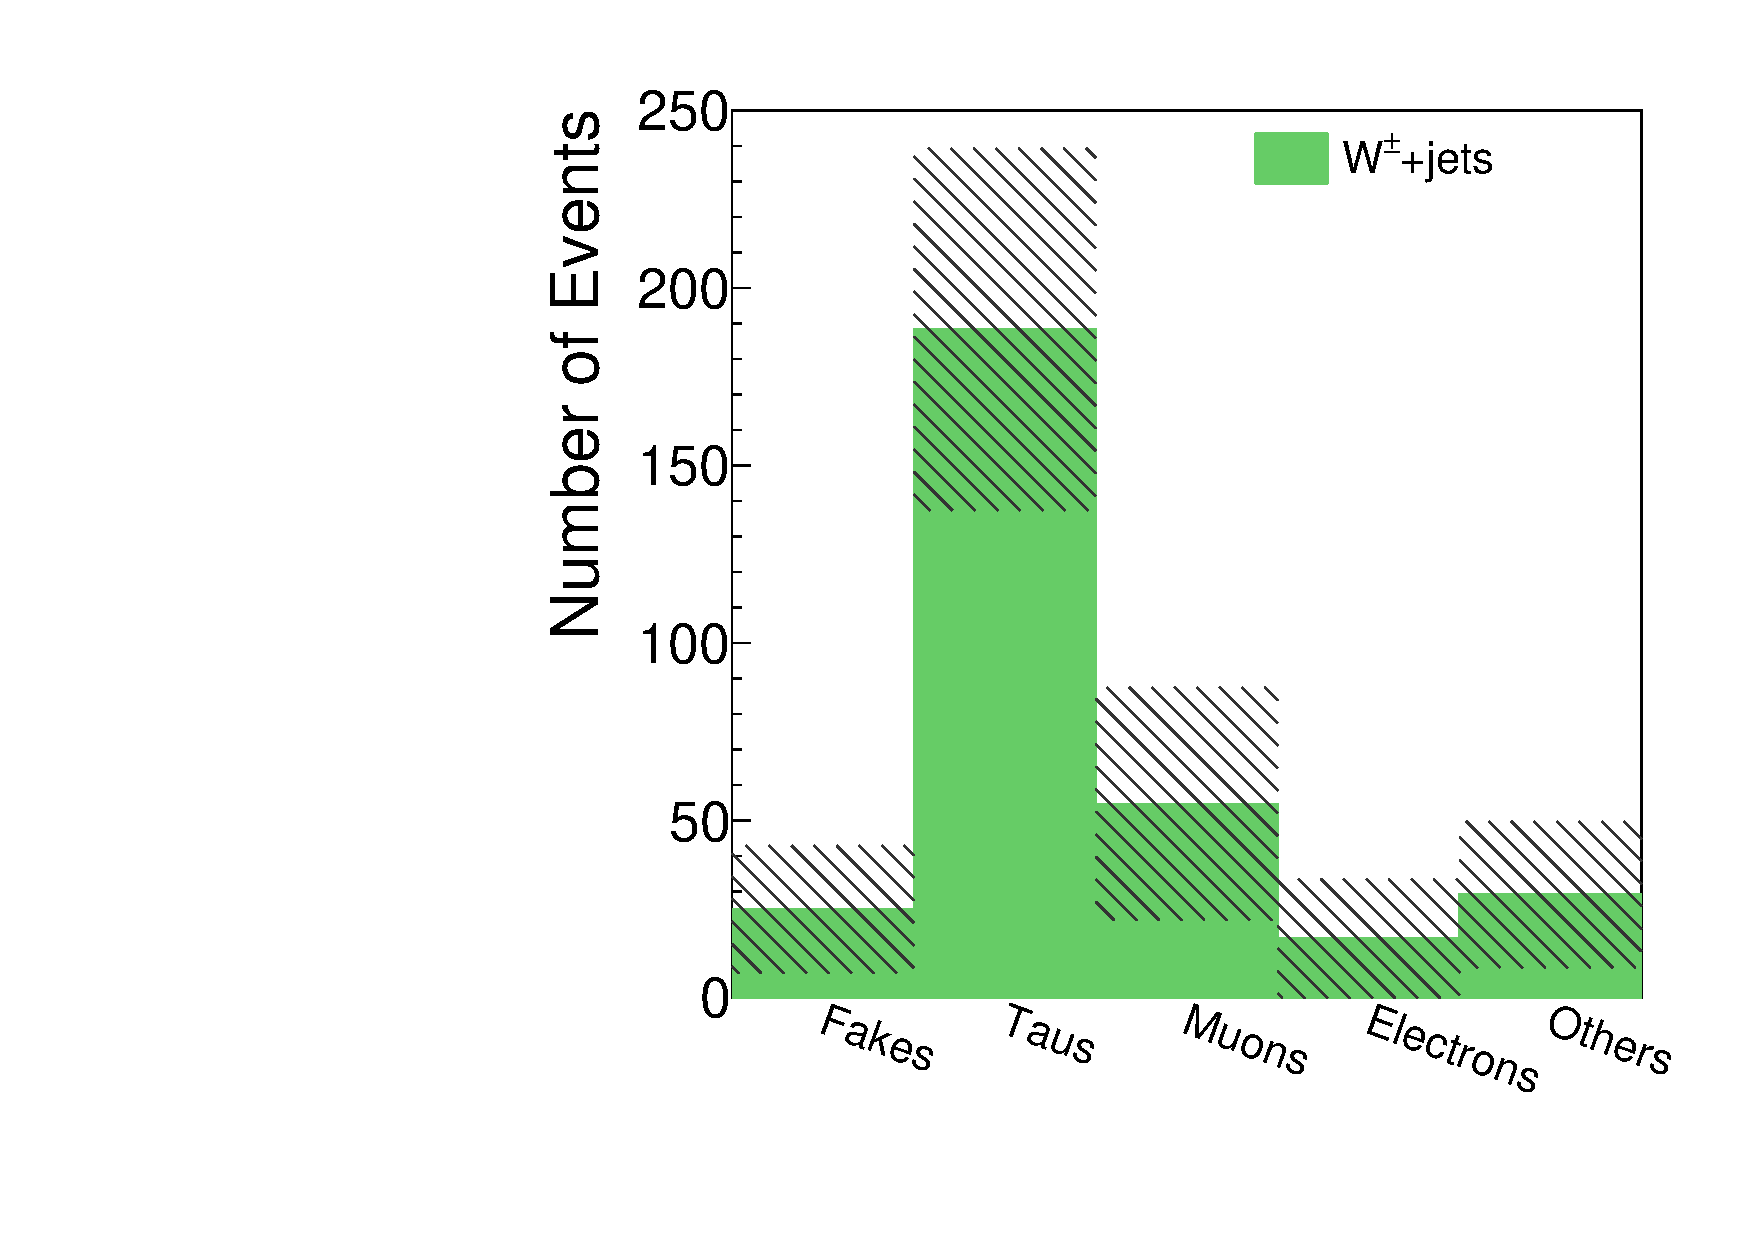
\includegraphics[width=0.49\textwidth]{figures/analysis/htrackgenParticleSmallRange_lin_chiTracksfullSelectionTrigger.pdf}
    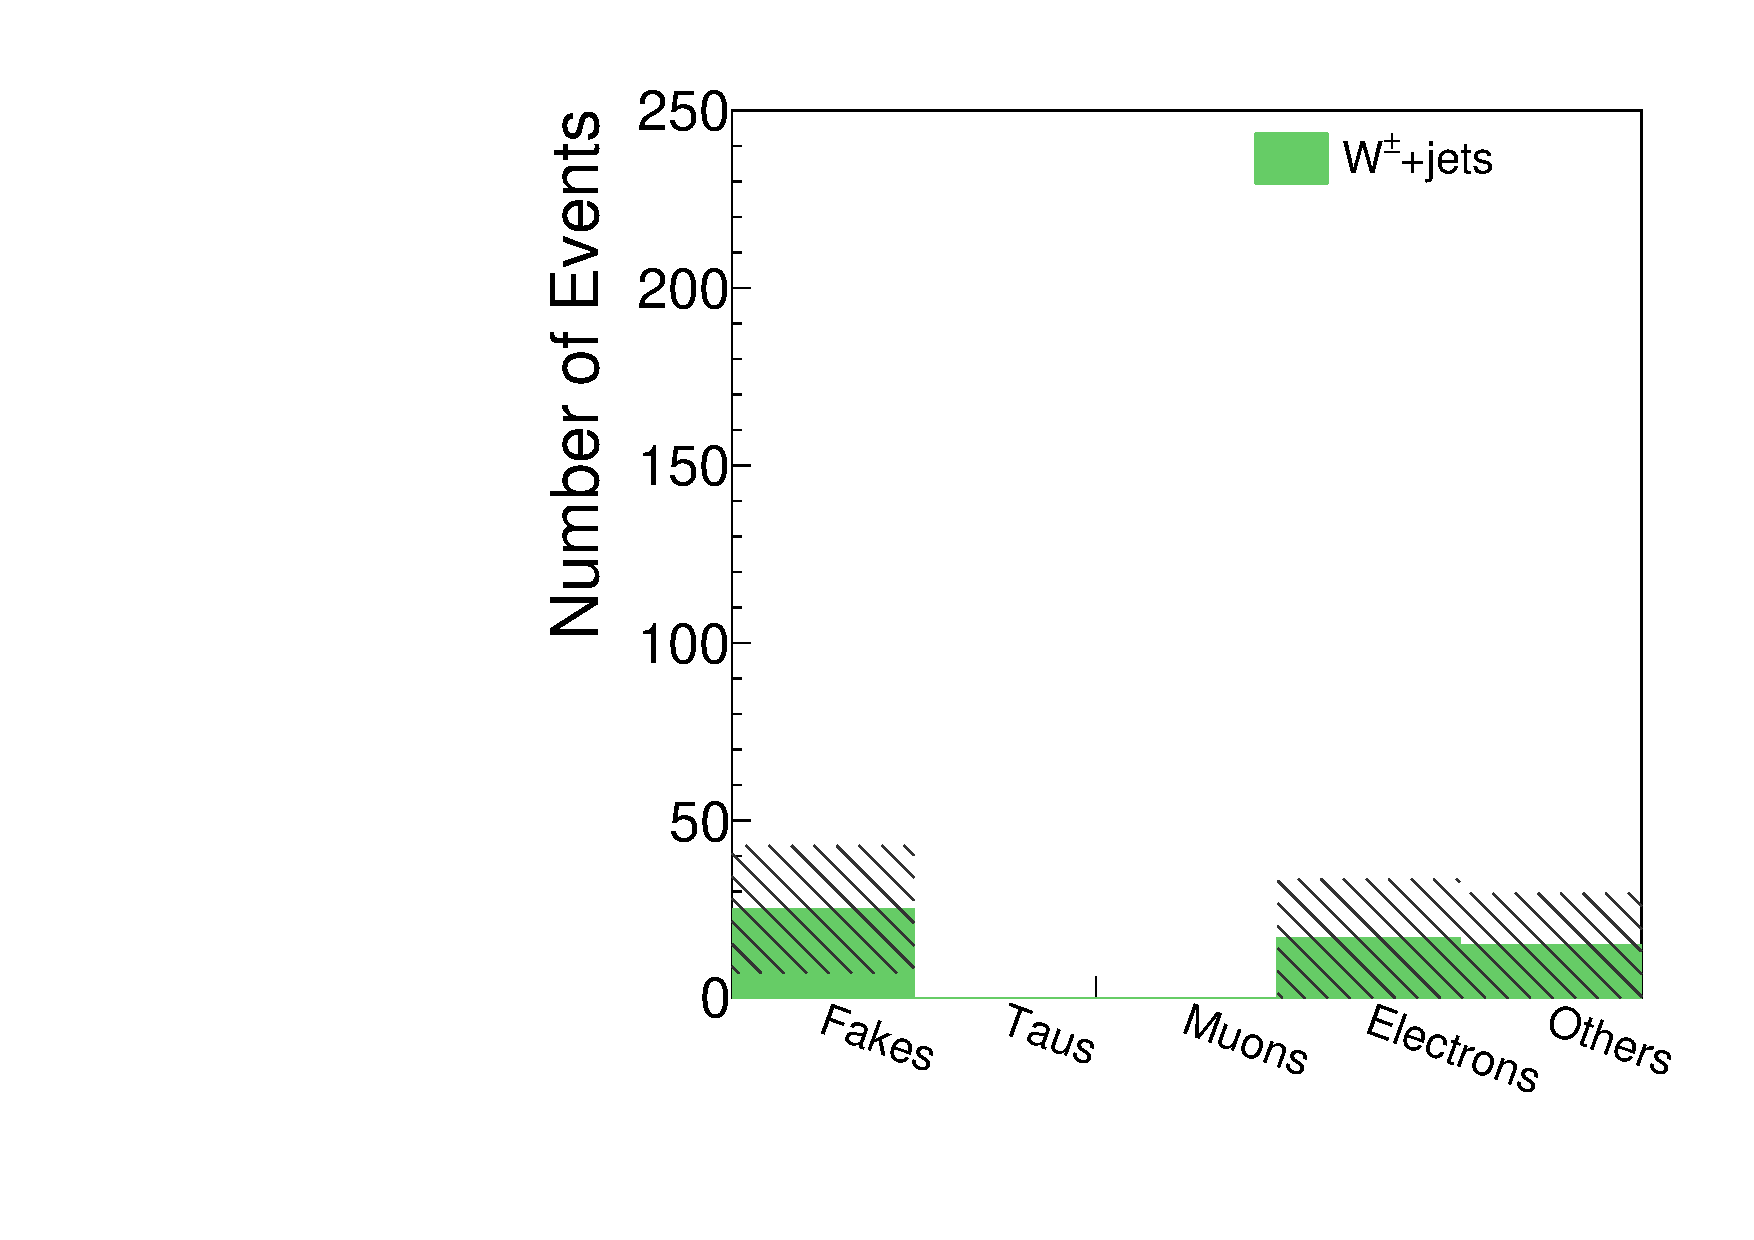
\includegraphics[width=0.49\textwidth]{figures/analysis/htrackgenParticleSmallRange_lin_chiTracksfullSelectionPlusIasTrigger.pdf}
  \end{tabular}
  \caption{bla bla}
  \label{fig:BkgComposition}
\end{figure}
This composiiton can change significantly when imposing further selection cuts on \pt and \ias.
This, however, will be addressed during the optimisation procedure.
To get a feeling how the composition of the background is affected by further cuts on one of the main variable \ias, 
the background composition is shown in Fig~\ref{fig:BkgComposition} with the analysis selection plus an additional \ias cut of 0.5.
As can be already seen in this figure the fake background becomes more important when apply also a selection on \ias, 
especially because the fake background is not only present in \WJets events but essentially in all Standard Model processes with missing energy. \\

Still, also the leptonic background can be important.
This is not possible to study with simulation because of the lack of statistics.
Additionally, when the simulation is not fully correct in simulating the operativeness of every single detector module, the simulation could highly underestimate the leptonic background.
Thus, a data based background estimation approach is needed.

\subsection{Leptonic background}
\label{sec:LeptonicBkg}

The leptonic background of the presented search is caused by non-reconstructed leptons which undergo hence the lepton veto selection.
However, at least a non-reconstructed electron or tau should in principle deposit enough energy in the ECAL that it can still be vetoed by the calorimeter isolation requirement.
As muons don't deposit much energy in the ECAL, this reason does not hold for them.
In the following, the sources of the three different leptonic backgrounds shall be charectized.

\subsubsection*{Electrons}
To avoid the background source from unreconstructed electrons, all tracks pointing to a dead or noisy ecal cells are vetoed, as described in the previous section.
By this selection, almost all electrons are efficiently rejected.
In the simulated \WJets sample only one simulated event remain which pass all candidate track selection criteria and where the candidate track can be matched to generator-level electron .
This event is visualised in Fig~\ref{fig:LostElectron}. 
\begin{figure}[!tb]
  \centering 
  \begin{tabular}{c}
    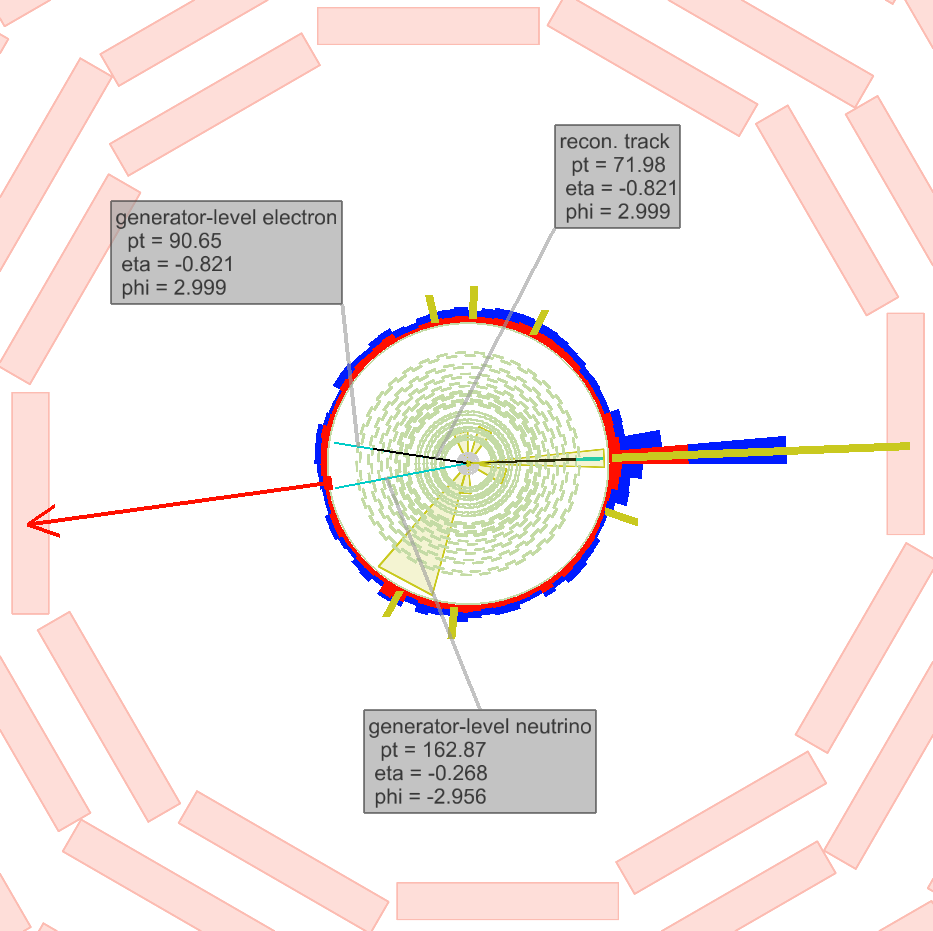
\includegraphics[width=0.49\textwidth]{figures/analysis/Electron_lumi_279317_event_111637553.png}
  \end{tabular}
  \caption{Visualization of an $W\rightarrow e\nu_e$ event contributing to the SM background. 
           In light blue the generator-level particles $e$ and $\nu_e$ of the $W$ decay are shown. 
           The $\nu_e$, only weakly interacting does not show any signature in the detector, whereas the electron ($\pt\simeq 90\gev$) leaves a track (black line) with \mbox{$\pt\simeq 70\gev$} in the tracker. 
           No ECAL energy deposits in the direction of the electron are visible. 
           This is caused by the fact that the corresponding ECAL energy deposits were not read out in this event.
           An ISR jet ($\pt\simeq 230\gev$) causes the \met (read arrow) in the event. }
  \label{fig:LostElectron}
\end{figure}
In this event to energy deposits in the ECAL are read out, which suggests, that this ECAL tower was neither working properly in 2012.
Additionally, electrons might do much bremstrahlung and as a effect can change the direction significantly, such that the deposited energy in the ECAL is not matched to the electron.

\subsubsection*{Taus}
The tau background is contributing through the hadronic decay of a tau lepton to one charged pion $\tau\rightarrow\pi^{\pm}\nu$.
Unreconstructed taus have typically large mismeasured \pt.
Because of nuclear interactions in the tracker, they have typically short tracks and therefore easily mismeasured \pt.
Additionnaly, the pion already looses energy in the tracker which opens up the possibility surviving also the calorimeter isolation selection.
Such an event is shown in Fig.~\ref{fig:LostTau}.
Unfortunately, due to the short length of the track, these events can sometimes also survive an \ias cut, because of possibly large $dE/dx$ fluctions.
\begin{figure}[!tb]
  \centering 
  \begin{tabular}{c}
    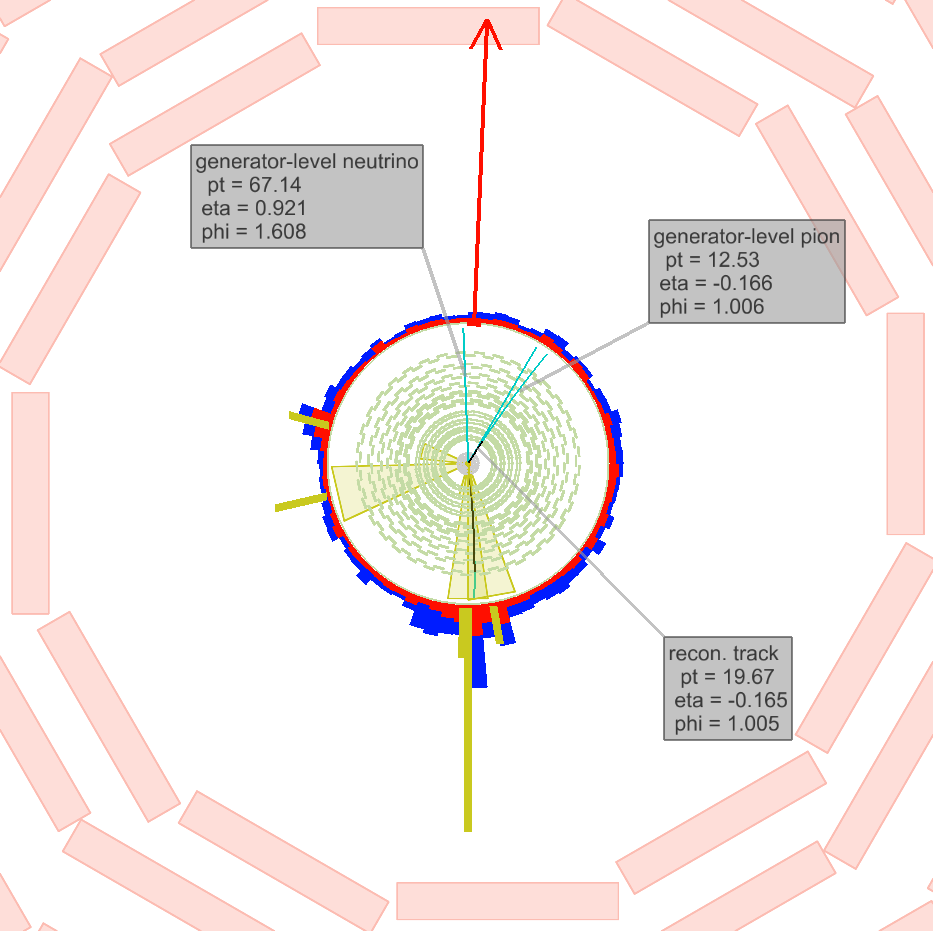
\includegraphics[width=0.49\textwidth]{figures/analysis/LostTau_Lumi_60133_Event_24033837.png}
  \end{tabular}
  \caption{Visualization of a $W^{+}\rightarrow \tau^{+}\nu_{\tau} \rightarrow \pi^{+} \nu_{\tau}$ event contributing to the SM background. 
           In light blue the generator-level particles $\pi^{+}$ and $\nu_{\tau}$ are shown.
           The reconstructed track (black line) is very short because the pion interacts with the tracker material via the strong force.}
  \label{fig:LostTau}
\end{figure}

\subsubsection*{Muons}
Muons can fail reconstruction when they are pointing torward a bad cathode strip chamber.
This is taken into account in the candidate track selection.
However, some of the muons still fail reconstruction when they fall within the gap between stations 0 and 1 of the DT system at $\eta=0.25$.
The muon reconstruction efficiency drops from around 99\% to a value of around 94\% as shown in~\ref{jessicathesis}. 
This possibility is illustrated in a simulated event shown in Fig~\ref{fig:LostMuon}.
\begin{figure}[!tb]
  \centering 
  \begin{tabular}{c}
    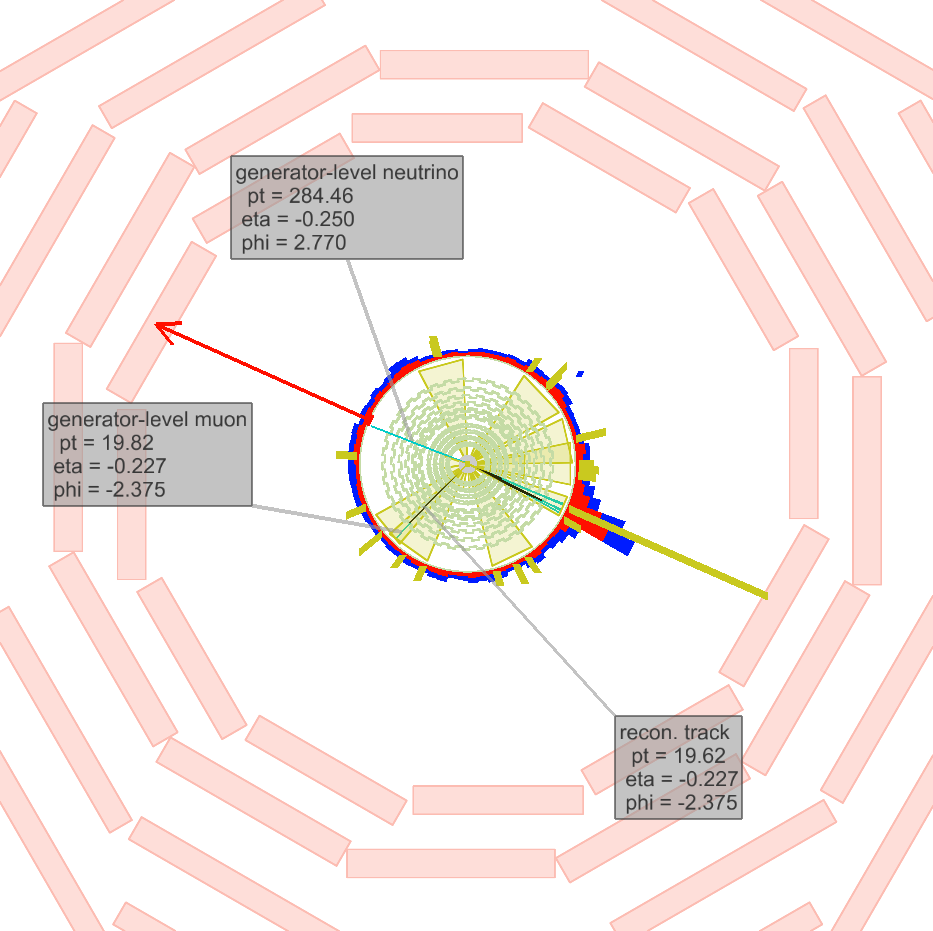
\includegraphics[width=0.49\textwidth]{figures/analysis/LostMuon_Lumi_357583_Event_142918834.png}
  \end{tabular}
  \caption{Visualization of an $W\rightarrow \mu\nu_{\mu}$ event contributing to the SM background. 
           In light blue the generator-level particles $\mu$ and $\nu_{\mu}$ of the $W$ decay are shown. }
  \label{fig:LostMuon}
\end{figure}
In~\ref{jessicastheisi} events are rejected when the track is pointing in a region of $0.15<|\eta|<0.35$.
In this search, this cut was omitted to maximise signal acceptance. 
Due to the additional selection in \ias, muons are easily efficiently supressed.
E.g. in the event example shown in Fig~\ref{fig:LostMuon}, the muon has an \ias value of about 0.02.\\


In general, all leptons are rather minimal ionizing, especially muons and pions.
Electrons can more easily interact with the shell electrons of the tracker material, but still the \ias spectrum is quickly decreasing compared to the signal.
To have the possibility to make an optimisation in the two main discriminating variables \pt and \ias, the background estimation methods are designed to work for all different \pt and \ias selection cuts.
\begin{itemize}
\item Show ias plot for electrons, muons, taus seperately!
\item Explain background estimation method
\item with fake background (should be metioned before the leptonic background!!!!!)
\end{itemize} 



%%%%%%%%%%%%%%%%%%%%%%%%%%%%%%%%%%%%%%%%%%%%%%%%%%%%%%%%%%%%%%%%%%%%%%%%%%%%%%%%%%%%%%%%%%%%%%%%%%%%%%%%%%%%%%%%%%%%%%%%%%%%%%%%%%%%%%%%%%%%%%%%%%%%%%%%%%%%%%%%%%%%%%%%%%%%%%%%%%%%
\subsection{Fake background}
\label{sec:FakeBkg}

\begin{itemize}
\item Show plot with fake rate in different samples
\end{itemize}

\subsection{Systematic uncertainties}
\label{sec:SysUncertaintiesBkg}


\begin{itemize}
\item Background consist of particles which make high energy deposits and are high pt
\item In general: Low background search
\end{itemize}


\newpage
%%%%%%%%%%%%%%%%%%%%%%%%%%%%%%%%%%%%%%%%%%%%%%%%%%%%%%%%%%%%%%%%%%%%%%%%%%%%%%%%%%%%%%%%%%%%%%%%%%%%%%%%%%%%%%%%%%%%%%%%%%%%%%%%%%%%%%%%%%%%%%%%%%%%%%%%%%%%%%%%%%%%%%%%%%%%%%%%%%%%
%%%%%%%%%%%%%%%%%%%%%%%%%%%%%%%%%%%%%%%%%%%%%%%%%%%%%%%%%%%%%%%%%%%%%%%%%%%%%%%%%%%%%%%%%%%%%%%%%%%%%%%%%%%%%%%%%%%%%%%%%%%%%%%%%%%%%%%%%%%%%%%%%%%%%%%%%%%%%%%%%%%%%%%%%%%%%%%%%%%%
\section{Optimization of search sensitivity}
\label{sec:Optimization}
\begin{itemize}
\item Show plots
\item show table
\item Include NlostOuter here, too
\end{itemize}

%%%%%%%%%%%%%%%%%%%%%%%%%%%%%%%%%%%%%%%%%%%%%%%%%%%%%%%%%%%%%%%%%%%%%%%%%%%%%%%%%%%%%%%%%%%%%%%%%%%%%%%%%%%%%%%%%%%%%%%%%%%%%%%%%%%%%%%%%%%%%%%%%%%%%%%%%%%%%%%%%%%%%%%%%%%%%%%%%%%%
\section{Statistical Methods/ Limit setting}
\label{sec:LimitSetting}

%%%%%%%%%%%%%%%%%%%%%%%%%%%%%%%%%%%%%%%%%%%%%%%%%%%%%%%%%%%%%%%%%%%%%%%%%%%%%%%%%%%%%%%%%%%%%%%%%%%%%%%%%%%%%%%%%%%%%%%%%%%%%%%%%%%%%%%%%%%%%%%%%%%%%%%%%%%%%%%%%%%%%%%%%%%%%%%%%%%%
\section{Results}
\label{sec:Results}
\begin{itemize}
\item Data cutflowtable
\item Tables with results
\item One plot (4 bins: Prediction and data)
\end{itemize}

%%%%%%%%%%%%%%%%%%%%%%%%%%%%%%%%%%%%%%%%%%%%%%%%%%%%%%%%%%%%%%%%%%%%%%%%%%%%%%%%%%%%%%%%%%%%%%%%%%%%%%%%%%%%%%%%%%%%%%%%%%%%%%%%%%%%%%%%%%%%%%%%%%%%%%%%%%%%%%%%%%%%%%%%%%%%%%%%%%%%
\section{Interpretation}
\label{sec:Interpretation}
\subsection{Systematic uncertainties of simulated signal samples}
\subsection{Exclusion limits}
\begin{itemize}
\item 1-d limits
\item 2-d limits
\end{itemize}

